\section{Durchführung}
\label{sec:Durchführung}
Der prinzipielle Aufbau des Versuchs besteht aus einem Reflexklystron, einem
Einweggleichrichter, einem Frequenzmesser und einem Abschwächer, wie in Abbildung
\ref{fig:aufbau} dargestellt ist.
\begin{figure}[H]
  \centering
  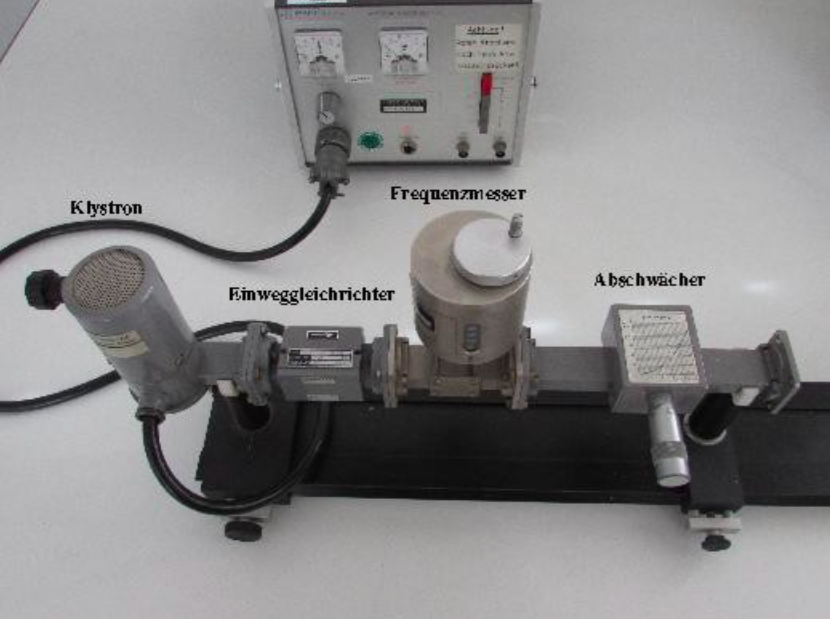
\includegraphics[height=9cm]{Aufbau.png}
  \caption{Versuchsaufbau \cite{skript}.}
  \label{fig:aufbau}
\end{figure}
Dieser Aufbau ist für alle Versuchsteile gleich und wird jeweils um die passenden
Bauteile ergänzt. Das Klystron dient hierbei zur Erzeugung der Mikrowellen und der
Gleichrichter verhindert, dass dieses durch reflektierte Wellen beschädigt wird.
Vor Beginn des Versuchs muss das Klystron zunächst für etwa eine Minute vorgeheitzt
werden.

\subsection{Untersuchung der Moden}
Zur Untersuchung der Moden wird das Klystron an das Oszilloskop angeschlossen, welches
die Moden im x-y-Betrieb darstellt. Zu diesem Zweck wird die Dämpfung auf etwa
$\SI{30}{\decibel}$ eingestellt. Auf der horizontalen Achse ist dabei die Reflektorspannung
dargestellt und auf der vertikalen Achse die Amplitude. Nun wird die Reflektorspannung
so eingestellt, dass die zu untersuchende Mode mittig auf dem Oszilloskop zu sehen ist.
Anschließend wird die Frequenz am Frequenzmesser so lange durchgestimmt, bis eine kleine
Ausbuchtung auf der parabelförmigen Mode zu sehen ist, die dann möglichst auf die
Spitze der Parabel gefahren wird. Nun werden die Reflektorspannung, die Amplitude und
die Frequenz notiert, zudem wird auch vermessen bei welcher Reflektorspannung der jeweils
linke und rechte Schwingungseinsatz mittig auf dem Oszilloskop dargestellt ist und die
entsprechenden Werte ebenfalls notiert. \\

\subsection{Bestimmung von Wellenlänge und Frequenz}
Um die Wellenlänge zu untersuchen wird hinter den grundlegenden Aufbau zusätzlich der
verschiebbare Stehwellendetektor und ein Kurzschluss angebaut, so dass die einlaufenden
Mikrowellen reflektiert werden und somit stehende Wellen im Hohlleiter bilden. Die Reflektorspannung
wird nun auf etwa $\SI{200}{\volt}$ eingestellt und die Dämpfung auf $\SI{20}{\decibel}$, mit einer
Modulation von $\SI{1}{\kilo\hertz}$. Die Messsonde wird daraufhin in ein Minimum des Ausschlags am SWR-Meter
gefahren und die Position notiert, anschließend wird auch das nächste Minimum detektiert. Aus dem
Abstand der beiden Minima lassen sich Wellenlänge und Frequenz berechnen.

\subsection{Bestimmung der Dämpfung}
Für diesen Versuchsteil wird hinter den Stehwellendetektor ein Abschluss angebaut. Die Verstärkung am
SWR-Meter wird bei sehr geringer Dämpfung nun so eingestellt, dass der Ausschlag auf der
unteren Skala bei $\SI{0}{\decibel}$ liegt. Die Dämpfung wird nun schrittweise so erhöht, dass
der Ausschlag bei $\SI{2}{\decibel}$, $\SI{4}{\decibel}$, $\SI{6}{\decibel}$, $\SI{8}{\decibel}$
und $\SI{10}{\decibel}$ liegt und die entsprechenden Stellungen der Mikrometerschraube des Dämpfungsgliedes
wird notiert, sowie auch die entsprechenden Dämpfungswerte die aus der Eichkurve resultieren.

\subsection{Untersuchung des Welligkeitsverhältnisses}
Zur Bestimmung des Welligkeitsverhältnisses wird zunächst zwischen Detektor und Abschluss ein
Gleitschraubentransformator eingebaut, welcher je nach Tiefe des Stiftes einen bestimmten
Anteil der Welle reflektiert. \\
Als erstes wird die direkte Methode verwendet, bei welcher das Stehwellenverhältniss direkt über die
Sonde gemessen wird. Dazu wird die Sonde zunächst in ein Maximum des Ausschlags, also einem minimalen
Wert gefahren und dieser Ausschlag dann auf 1,0 mittels Verstärkung eingestellt. Anschließend
wird die Sonde in das nächste Minimum des Ausschlags gefahren und der entsprechende Wert notiert.
Dieses Vorgehen wird jeweils für Stifttiefen von $\SI{0}{\milli\meter}$, $\SI{3}{\milli\meter}$,
$\SI{5}{\milli\meter}$, $\SI{7}{\milli\meter}$ und $\SI{9}{\milli\meter}$ wiederholt. \\
Eine weitere Methode ist die $\SI{3}{\decibel}$ Methode, für welche die Sonde ebenfalls zunächst in
ein Minimum gefahren wird, dessen Lage über die Stellung der Mikrometerschraube der Sonde notiert wird.
Die Tiefe des Gleitschraubentransformators sollte dabei $\SI{9}{\milli\meter}$ betragen.
Der Wert des Minimums wird über Verstärkung auf $\SI{3}{\decibel}$ auf der unteren
Skala eingestellt. Daraufhin wird die Sonde langsam nach links gefahren, bis der Ausschlag einen
Wert von $\SI{0}{\decibel}$ erreicht und die Stellung notiert. Analog wird auch für den Bereich rechts des Minimums
vorgegangen. Es sollte außerdem erneut die Wellenlänge bestimmt werden, da das Klystron während des
Versuchs gegebenenfalls verstimmt wird. \\
Das Stehwellenverhältniss lässt sich zudem auch über die Dämpfung bestimmen mit der sogenannten Abschwächer
Methode. Hier sollte die Tiefe des Gleitschraubentransformators ebenfalls bei $\SI{9}{\milli\meter}$ liegen.
Auch hier wird die Sonde zunächst in ein Minimum gefahren und die Verstärkung so eingestellt, dass der Ausschlag bei
einer Dämpfung von $\SI{20}{\decibel}$ am Dämpfungsglied genau $\SI{3}{\decibel}$ auf der unteren Skala
beträgt. Nun wird mit der Sonde das nächstgelegende Maximum des Ausschlags detektiert, wobei die
Dämpfung während des Verschiebens der Sonde stets so angepasst wird, dass das SWR-Meter Werte innerhalb des
Messbereichs der Skala anzeigt. Sobald das Maximum detektiert ist, wird es über Verstellen der Dämpfung
auf einem Wert von ebenfalls $\SI{3}{\decibel}$ gelegt und anschließend die Stellung der Mikrometerschraube
des Dämpfungsgliedes notiert, sowie die entsprechende Dämpfung aus der Eichkurve.
